\chapter{Robust motion planning with accuracy optimization based on learned sensitivity metrics}[]
\markboth{Robust MP with accuracy optimization based on learned sensitivity metrics}{}% To set left/right header
% \localtableofcontents

To overcome some of the aforementioned problems, the sensitivity-aware motion planner (SAMP) proposed in~\cite{cSAMP} exploits the derivation of uncertainty tubes of \cite{cTube}, based on the so-called \emph{closed-loop sensitivity}~\cite{cPi,cTh}.
This approach is applicable to any controller and robot model, taking into account parametric uncertainties. 
However, this planner suffers from the high computational cost of computing the uncertainty tubes.
Moreover, SAMP and the aforementioned methods focus on computing robust trajectories but do not consider the problem of \emph{also} minimizing uncertainty tubes at a desired location for increasing the accuracy of specific tasks (e.g., insertion, grasping).

\begin{figure} [t]
    \centering
    \subfloat[\centering Robust motion planning]{{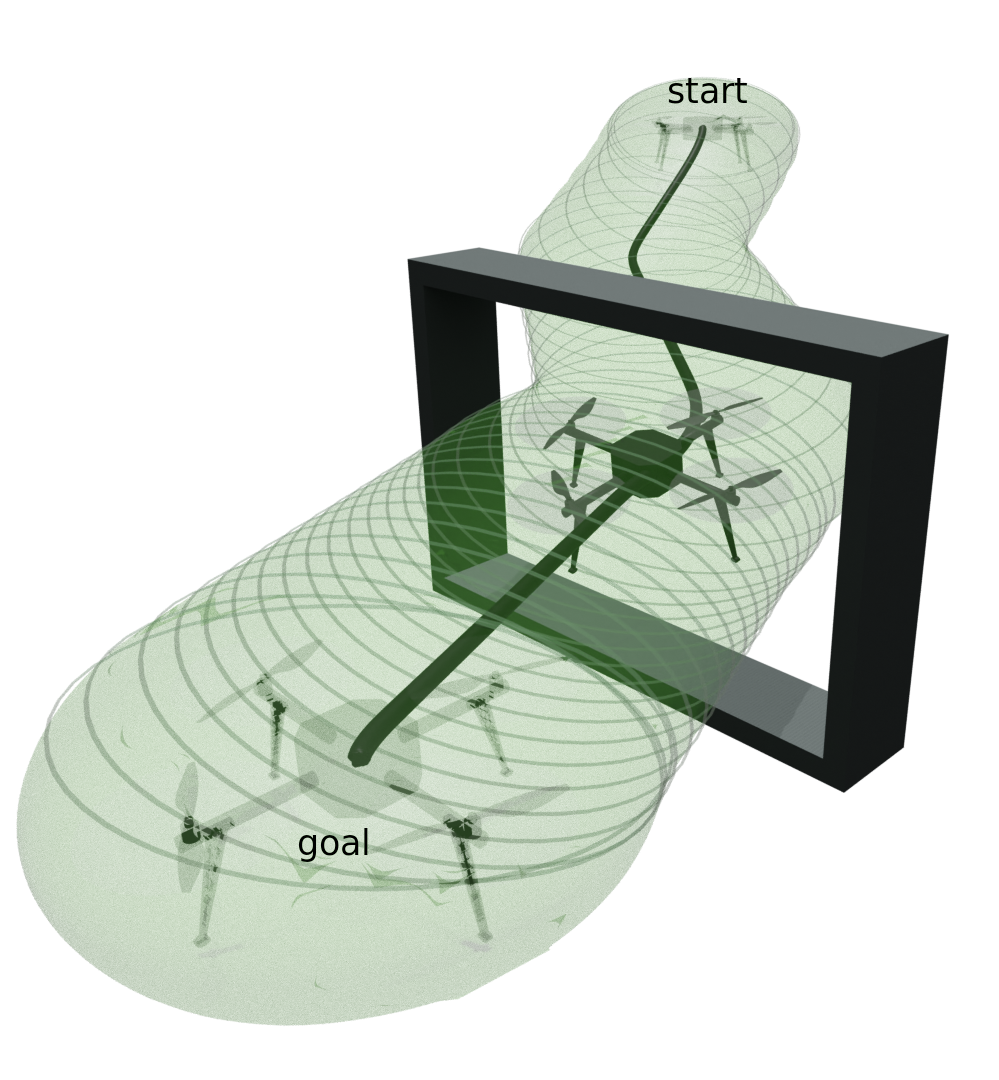
\includegraphics[width=0.4\linewidth]{figures/robust_accurate/topFig_tube.png} }\label{fig: fig1robust}}%
    \subfloat[\centering Accuracy optimization]{{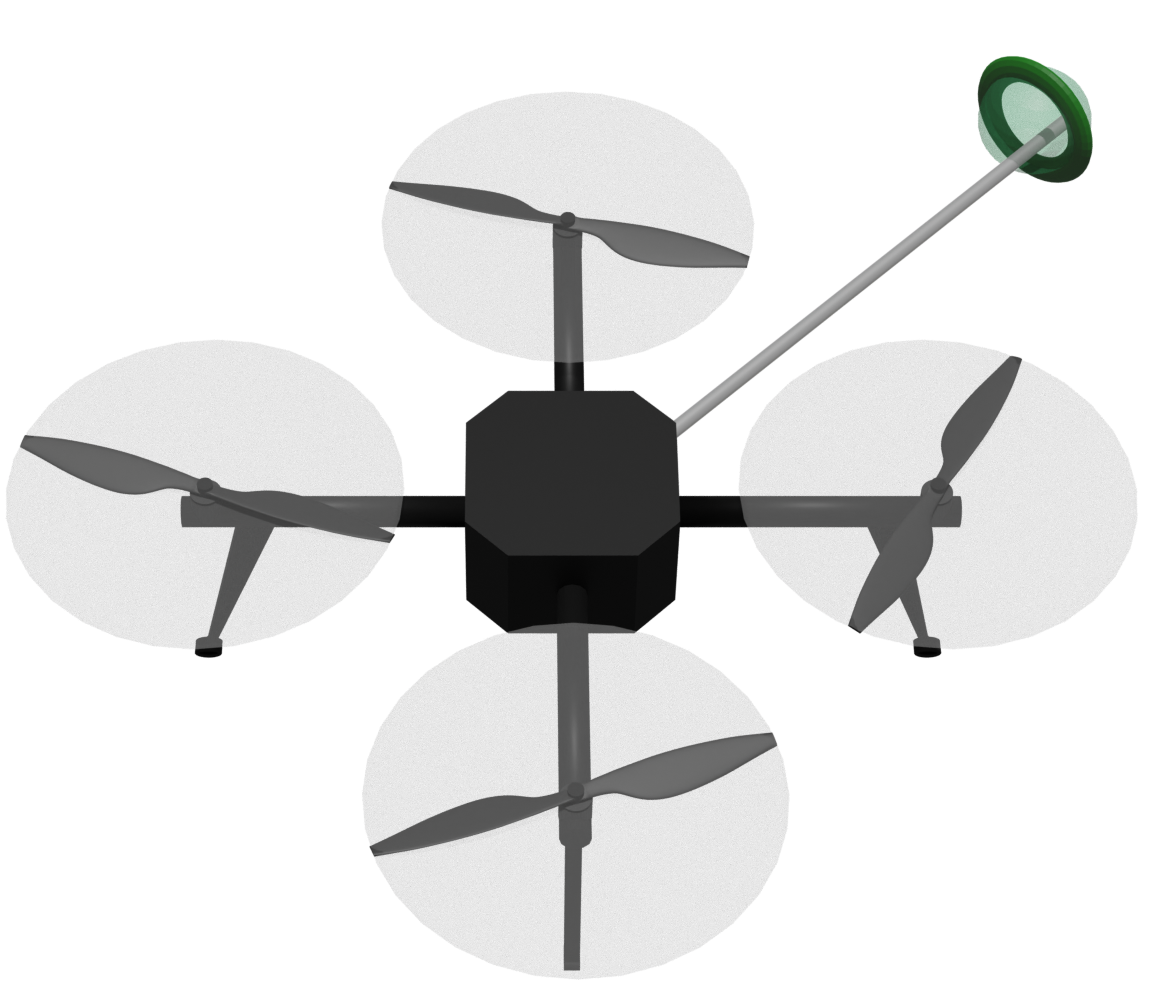
\includegraphics[width=0.4\linewidth]{figures/robust_accurate/ring_success.png} } \label{fig: fig1acc}}%
    \caption{
    Two scenarios considered for the experimental validation of the proposed method:
    (a) Robust navigation of a drone through a narrow window. (b) Precision in-flight `ring catching' task, where the uncertainty on the position of the perch end-effector is minimized to successfully accomplish the task.
    A video of the experiments is available at: \href{https://laas.hal.science/hal-04642257}{https://laas.hal.science/hal-04642257}}%
    \label{fig: Missed and succes}%
\end{figure}

With respect to these considerations, the contribution of this paper is twofold:
(i) We propose a computationally efficient version of the SAMP algorithm,
relying on a Gated Recurrent Unit neural network (GRU)\cite{cGRU} (see Chap.~\ref{chap:NN}), which quickly and accurately estimates time-varying uncertainty tubes and control input profiles along trajectories.
We present a general way of incorporating this type of network into a sampling-based tree planner in order to predict the uncertainty tubes and control inputs along trajectories. 
(ii) On the basis of this new planner, 
we propose a comprehensive framework that not only plans robust trajectories but also locally optimizes them together with the controller gains to maximize accuracy at some desired states of the planned trajectory for any system/controller.

Fig.~\ref{fig: Missed and succes} illustrates the application to a quadrotor model in two different experimental scenarios involving uncertain parameters affecting the robot model (see Sect.~\ref{sec:SimuResults}): (i) a robust navigation through a narrow window;
(ii) an in-flight ring-catching task demonstrating the robustness and accuracy of the proposed framework. 

% Sect.~\ref{sec:RASAMP} provides an overview of our planning framework to generate robust and accurate trajectories.
% Sect.~\ref{sec:RSAMP} shows how to integrate the sensitivity learning method within a sampling-based motion planner, while Sect.~\ref{sec:AOptim} explains the accuracy optimization stage.

\section{Robust and accurate planning framework}\label{sec:RASAMP}

The method consists of two stages: $(i)$ first, it generates a robust trajectory based on a Robust Sensitivity-Aware Motion Planner (R-SAMP) -- explained in Sect.~\ref{sec:RSAMP} -- that utilizes the GRU-based computation of the uncertainty tubes; $(ii)$ second, it optimizes the accuracy at some given states along this trajectory by minimizing the size of the uncertainty tubes at these locations.
The motivation behind the second stage is to improve the accuracy of the planned robust trajectory for tasks -- e.g., pick-and-place or insertion tasks -- where minimizing the deviation from the nominal trajectory is important only at specific designed locations, as for picking the ring in Fig.~\ref{fig: Missed and succes}.

The pseudo-code of RA-SAMP (Robust and Accurate Sensitivity-Aware Motion Planner) is presented in Alg.\ref{alg:RA-SAMP}. 
It takes as input (line 1) a list of desired states $list_{d} = (q_{d}^0, \dots, q_{d}^n)$ for which the accuracy should be optimized, and the initial controller gains vector $k_{c}^{init}$ considered constant all along the trajectory.

\begin{algorithm}[h]
\caption{RA-SAMP [$list_{d}, k_{c}^{init}$]}\label{alg:RA-SAMP}
\begin{algorithmic}[1]
\State $\pi_d^{tot} \gets \emptyset;$
\For {($i=1;\ i< len(list_{d});\ i=i+1$)}
    \State $\pi_d^{tot} \gets \pi_d^{tot} + $R-SAMP$(list_{d}(i-1),list_{d}(i));$
\EndFor
\State $\left \{ \pi_d^{tot}, k_{c}^{opt} \right \} \gets $A-Optim$(list_{d},\pi_d^{tot}, k_{c}^{init});$
\State \textbf{return} $\left \{ \pi_d^{tot}, k_{c}^{opt}  \right \}$;
\end{algorithmic}
\end{algorithm}

The first step of the algorithm consists of generating robust trajectories ($\pi_d^i$) between successive desired states in the list (line 3 of Alg.~\ref{alg:RA-SAMP}) by means of a robust sensitivity-aware motion planner called R-SAMP (explained in Sect.~\ref{sec:RSAMP}) that uses our learning approach.
These trajectories are concatenated into a global one $\pi_d^{tot}$, connecting all the desired states of $list_{d}$ (lines 2-5 in Alg.~\ref{alg:RA-SAMP}). 

The trajectory from R-SAMP is locally modified by A-Optim (line 6 in Alg.~\ref{alg:RA-SAMP}), aiming at optimizing the accuracy at specific desired states along the trajectory. 
This algorithm iteratively samples both the trajectory from R-SAMP and the controller gains, adjusting the former to minimize uncertainty at these states. 
Indeed, as demonstrated in \cite{AliIROS}, optimizing both factors concurrently results in minimizing the uncertainty.
The algorithm produces two offline outputs: $(i)$ a robust desired trajectory $\pi_d^{tot}$ optimized for accuracy at the desired states, and $(ii)$ the optimized controller gains vector $k_{c}^{opt}$, considered constant throughout the trajectory.

\subsection{Robust Sensitivity-Aware Motion Planner}\label{sec:RSAMP}

This section explains how the learned uncertainty tubes can be incorporated into any sampling-based tree planner in order to obtain a robust sensitivity-aware motion planner (R-SAMP).
As highlighted before, a key challenge in computing such tubes for a given trajectory lies in the high computational cost of numerically integrating the dynamics of $\bPi(t)$ and $\bTheta(t)$.
Additionally, when extending the tree and computing these sensitivity matrices, various initial conditions (e.g. initial control input, $\bPi_0$, etc.) must be embedded in the tree nodes.

We solve this problem thanks to the GRU network, which naturally encodes  this information in its ``memory'' terms, i.e., the so-called hidden state (see \cite{cGRU}).
An interesting feature of the algorithm is to leverage this latent state to embed the initial conditions into each node. This enables the reuse of the updated initial conditions for predictions in future extensions.
Note that a hidden state $h$ is unique according to its parent.
Therefore, its use is only applicable to tree-based planners, where each node has a single parent.
We show in Alg.~\ref{alg:ExtensionExample} how to incorporate this hidden state and tube predictions for the case of a standard RRT planner \cite{cRRT} with the pseudocode of the R-SARRT algorithm, as a particular instance of an R-SAMP planner. 
Note that the use of this hidden state and tube predictions can be similarly applied to other tree-based planners. For instance, in the results presented in Sect.~\ref{sec:RobustPlanSimu}, we used a robust RRT$^*$ implementation denoted R-SARRT$^*$.

First, R-SARRT performs the standard RRT procedure (lines 1-5) that produces a local desired trajectory $\pi_d$ between a sampled state (${q}^{rand}$) and its nearest state (${q}^{near}$) in the tree. 
Then, as the tubes are only valid around the nominal trajectories, which may differ from the desired ones depending on the controller performance, the nominal trajectory ($\pi_{n}$) is computed by the SimulateExecution function (line 6).
It corresponds to the simulated tracking in closed-loop of the desired trajectory ($\pi_d$) to be robustly checked by the system under the nominal parameters (i.e. $\p = \p_c$).
Next, the starting hidden state (as for $h_{0}$ of the GRU) is recovered from the tree node (line 7).
Such initial condition is used together with the above-mentioned nominal trajectory by the GRU that returns all the radii and the control inputs profiles ($\Rq,\Ru,\u$), together with the final hidden state $h_{F}$ to be reused as initial condition in subsequent iterations (line 8).
Then, for each state of the nominal trajectory $\pi_{n}$, the function \emph{IsRobust} (line 9) performs a robust collision checking by using the uncertainty radii, and tests if the inputs are within the admissible bounds that the system can exert.
If the extension is valid, the final state of the desired trajectory is inserted in the tree as a new node, embedding at the same time the final hidden state $h_{F}$ to be reused as initial condition in next iterations (line 10-12).
Finally, the algorithm returns a global trajectory connecting ${q}^{init}$ and ${q}^{goal}$ if one exists in the tree (lines 15).

\begin{algorithm}[t]
\caption{R-SARRT [$q^{init}, q^{goal}$]}\label{alg:ExtensionExample}
\begin{algorithmic}[1]
\State $T \gets$ InitTree$({q^{init}});$
\While{\textbf{not} StopCondition$(T, {q^{goal}})$}  
\State ${q^{rand}} \gets $Sample()$;$
\State ${q^{near}} \gets$ Nearest$(T,{q^{rand}});$
\State $\pi_d \gets$ Steer$({q^{near}},{q^{rand}});$
\State $\pi_{n} \gets $SimulateExecution$(\pi_d);$
\State $h_{0} \gets $GetNodeConditions$({q^{near}});$
\State $\left \{\Rq,\Ru,\u, h_{F} \right \} \gets $GRU$(\pi_d,h_{0});$
\If {$IsRobust(\Rq,\Ru,\u, \pi_{n})$}
        \State SetNodeConditions$({q^{rand}}, h_{F});$
        \State AddNewNode$(T, {q^{rand}});$
        \State AddNewEdge$(T, {q^{near}}, {q^{rand}});$
\EndIf
\EndWhile
\State \textbf{return} GetTrajectory$(T, q^{init}, q^{goal})$;
\end{algorithmic}
\end{algorithm}

\subsection{Robust local accuracy optimization \emph{(A-Optim)} }\label{sec:AOptim}

\subsubsection{Cost function}

The application of a local optimization method at this level is justified by the cost function considered in order to optimize the accuracy at desired states. 
Indeed, the cost of a trajectory $\pi$ is defined as:
\begin{equation}\label{eq: cost}
    c(\pi) = w_1\mathbb{E}[L] + w_2\mathbb{V}[L], \quad L = \left[\lambda_{0} ... \lambda_n \right]
\end{equation}
with $\mathbb{E}[L]$ and $\mathbb{V}[L]$ the mean and the variance of $L$, where $\lambda_k$ is the p-norm of the radii of interest in the $k$-th state in the $list_{d}$ of Sect.\ref{sec:RASAMP}, and $w_1, w_2$ are user-defined weigths.
The variance is considered in this cost function so that the minimization of a radius at a given point does not lead to the growth of another radius at another waypoint.
This function is neither additive (i.e., considering two trajectories ($\pi_{1}, \pi_{2}$), the cost of their concatenation $c(\pi_{1}|\pi_{2}) \neq c(\pi_{1}) + c(\pi_{2})$), nor monotonic. Therefore, it is unsuitable for global optimization using sampling-based motion planners like \cite{cRRT,cRRTstar}, since they require additive and monotonic objective functions.
Given that we do not have the analytic expression of the cost function derivatives, the accuracy optimization of A-Optim has to be performed by a derivative-free method. In this work, we simply used a robust version of the random shortcut algorithm~\cite{cShortcut} that performs robust collision checks (as in Alg.~\ref{alg:ExtensionExample}) to maintain the robustness of the initial trajectory computed by the R-SAMP planner.

\subsubsection{Methods}

\begin{enumerate}
    \item Shortcut
    \item ExtendedShortcut
    \item STOMP
    \item NL COBYLA
\end{enumerate}

Mentionned that maybe consider only a subpart of the trajectory before the accuracy waypoints might be better, only few time steps impact it.
Sampling for ExtendedShortcut maybe adaptive according to the difficulty of the convergence.

%%%%%%%%%%%%%%%%%%%%%%%%%%%%%%%%%%%%%%%%%%%%%%%%%%%%%%%%%%%%%%%%%%%%%%%%%%%%%%%%%%%%%%%%%%%%%%%%%%%%
\section{Simulation results} \label{sec:SimuResults}

This section first presents results showing the quality of the learning-based uncertainty tubes prediction and its high efficiency when used for robust motion planning. 
Then, we show the ability of the proposed R-SAMP\footnote{Code available at: \href{https://gitlab.laas.fr/CAMP}{https://gitlab.laas.fr/CAMP}} planning approach to generate robust 
and accurate trajectories for the two experimental scenarios illustrated in Fig.~\ref{fig: Missed and succes}.

%%%%%%%%%%%%%%%%%%%%%%%%%%%%%%%%%%%%%%%%%%%%%%%%%%%%%%%%%%%%%%%%%%%%%%%%%%%%%%%%%%%%%%%%%%%%%%%%%%%%
\subsection{Learning-based tube computation} \label{sec:NNresult}

The performance of the method presented in Chap.~\ref{chap:NN} and apply to a sampling based algorithm is illustrated in Fig.~\ref{fig: NN pred} that depicts the norm of predicted vector components for a 300-state trajectory part of the tree.
\todomarker[]{POlish: Note that the predictions are only valid for the parameter maximum range $\delta\p$ chosen during the generation of the training set, and that the model is trained for given values of the controller gains.
Also, learning optimal controller gains is left to future work, as it would require additional work on database generation and data annotation, the A-Optim method cannot benefit from it.}


\begin{figure} [t]
    \centering
    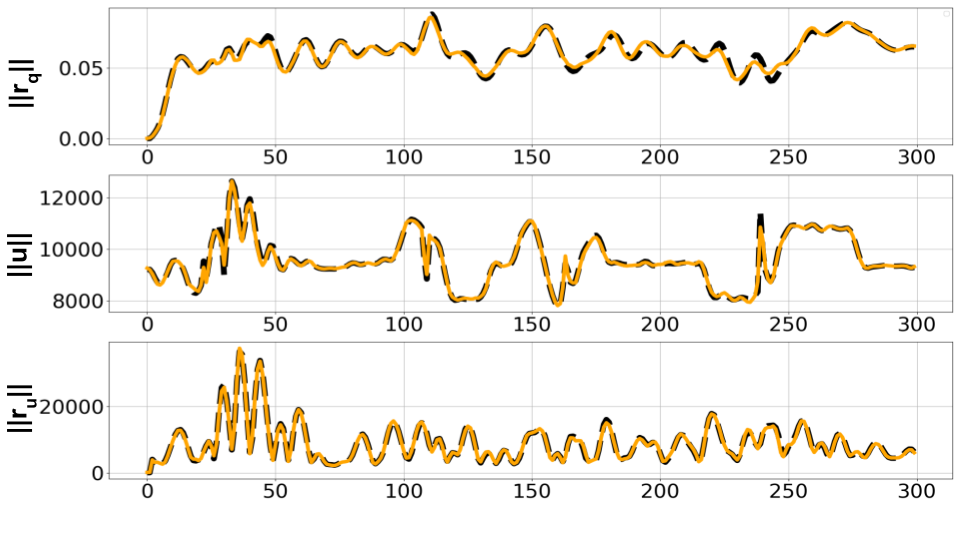
\includegraphics[width=0.8\linewidth]{figures/robust_accurate/PredNorm.png} 
    \caption{Example of GRU predictions along a trajectory (orange) against true values (back). $||\Rq||, ||\u||$ and $||\Ru||$ refer to the norm of their respective vector components. $||\Rq||$ is expressed in $m$, and control input associated values ($||\u||,||\Ru||)$ are squared propeller speeds [(rad/s)²].}%
    \label{fig: NN pred}%
\end{figure}

\begin{figure} [!t]
    \centering
    \subfloat[\centering RRT]{{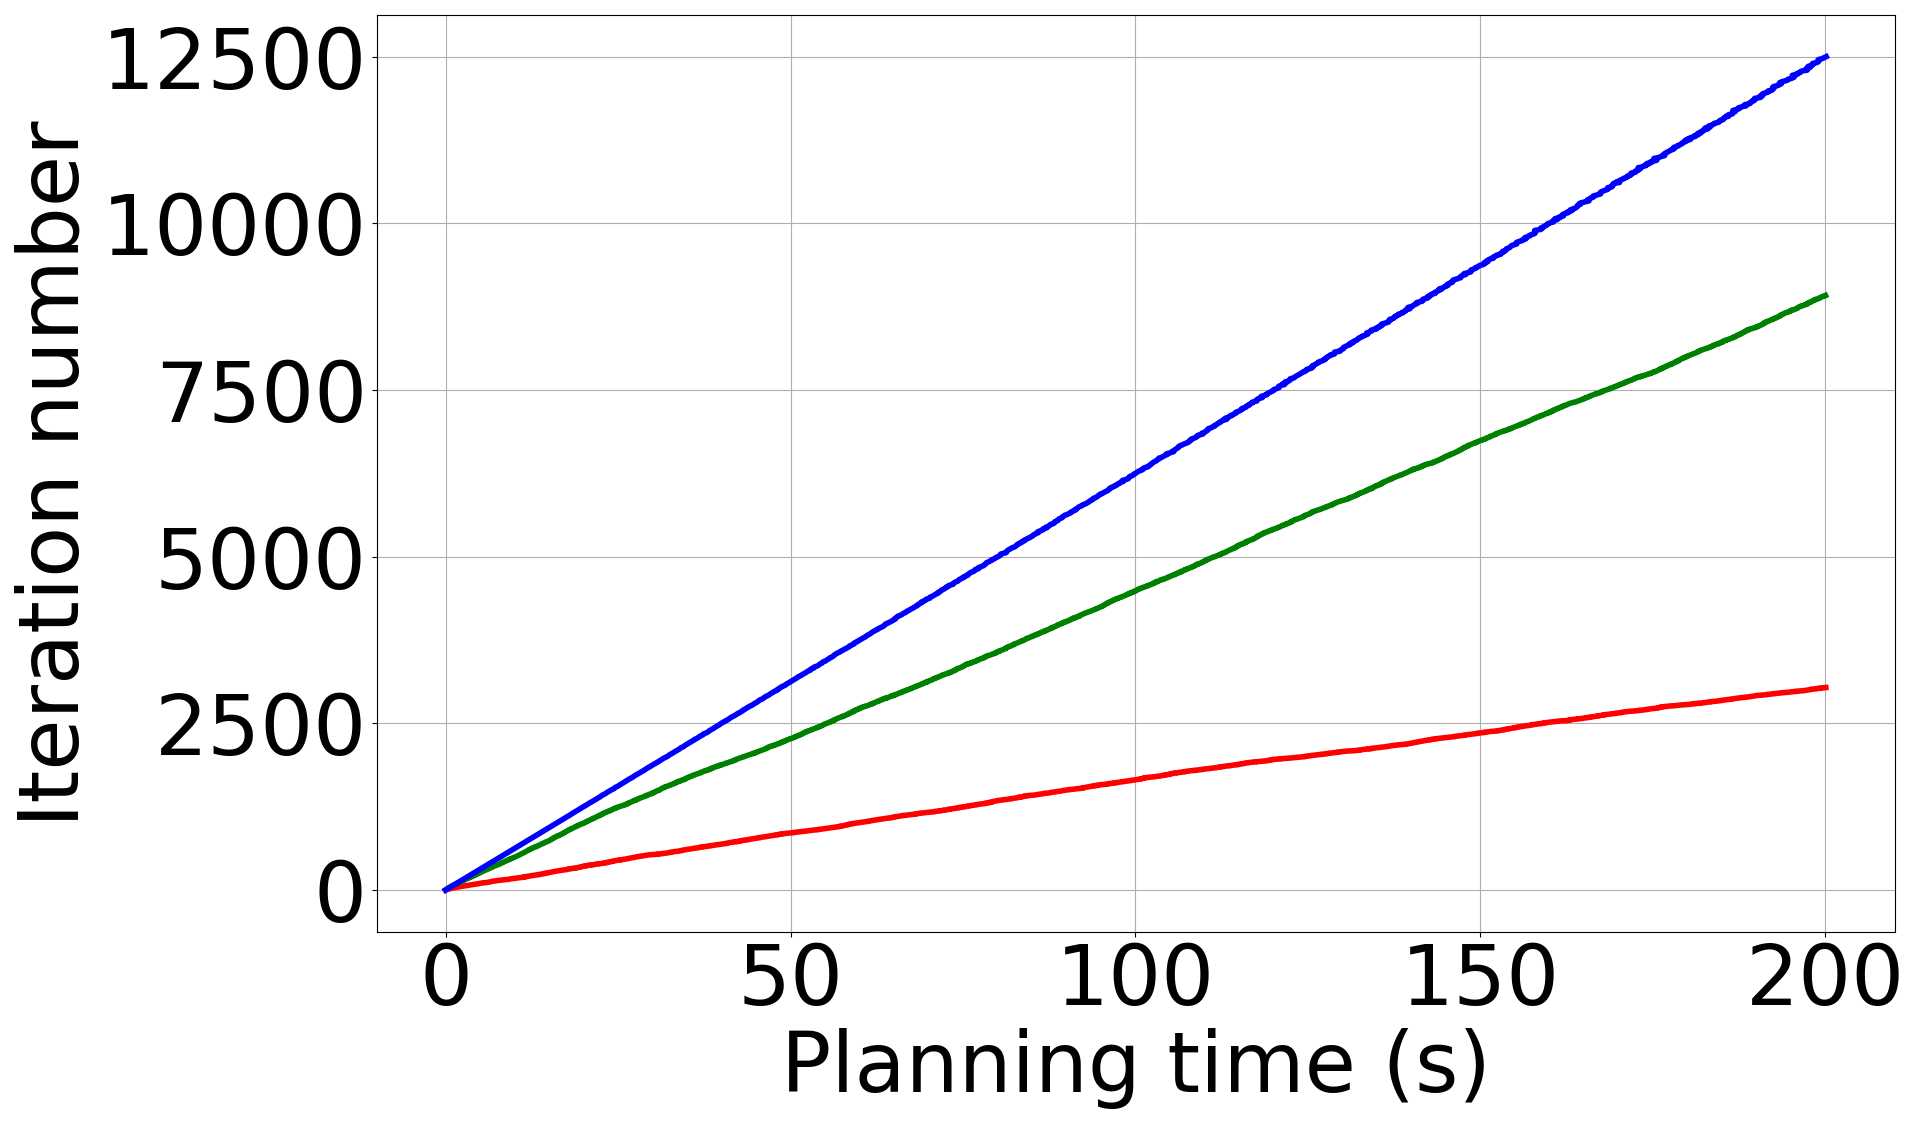
\includegraphics[width=0.4\linewidth]{figures/robust_accurate/iterations_RRT_new.png} }}%
    \subfloat[\centering RRT$^*$]{{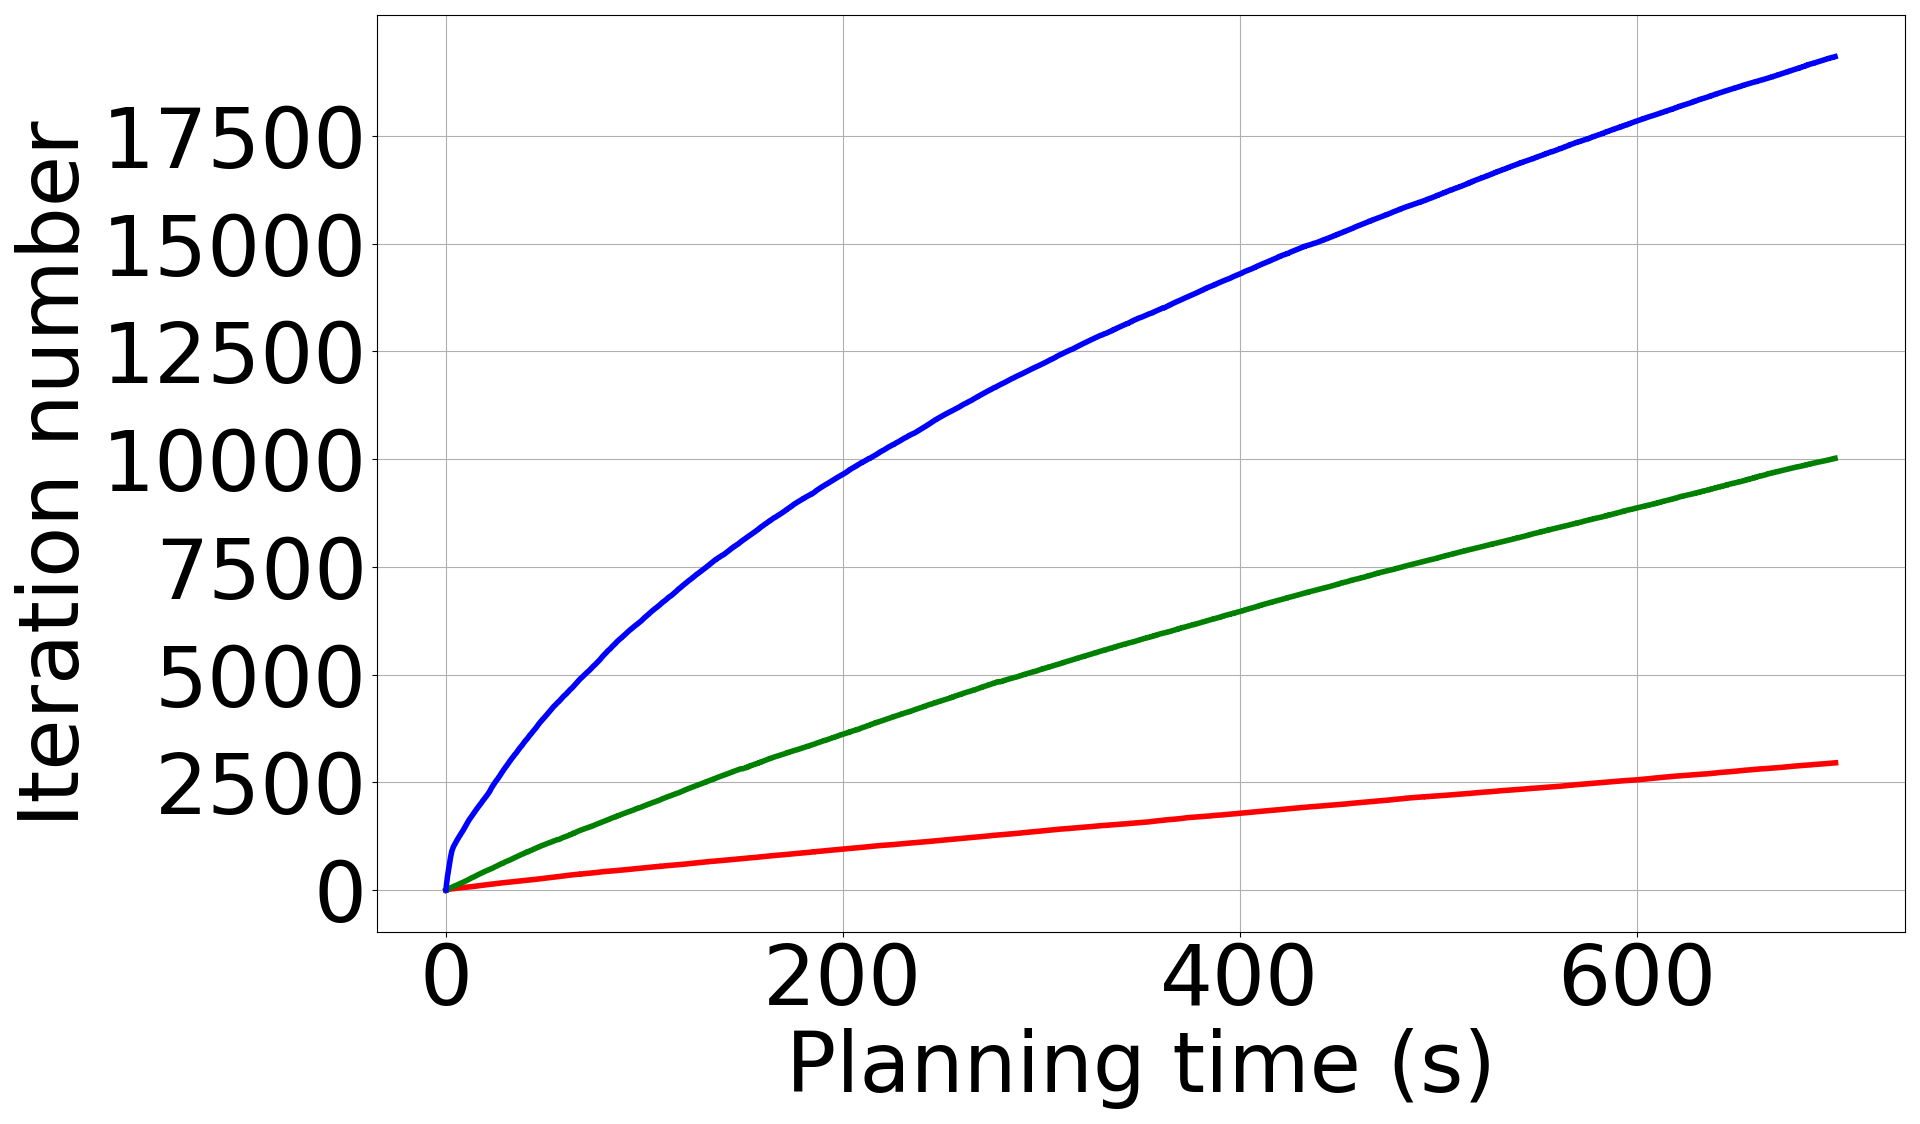
\includegraphics[width=0.4\linewidth]{figures/robust_accurate/iterations_RRTstar_new.png} }}%
    \caption{Number of (a) RRT / (b) RRT$^*$ iterations as a function of planning time in an obstacle-free environment using the standard (non-robust) RRT/RRT$^*$ implementation (blue), compared to robust versions using the GRU-based tube prediction (green) or the integration of the dynamics of $\bPi$ (red), as done in \cite{cSAMP}.}%
    \label{fig: NNTime}%
\end{figure}

\todomarker[]{ADD profiling ODEs vs learning}

Fig.~\ref{fig: NNTime} shows the significant performance improvement of using this learning-based prediction within a sampling-based tree planner for checking the robustness of the local tree expansions (see Alg.~\ref{alg:ExtensionExample}), against the previous version \cite{cSAMP} that directly integrates the $\bPi$ dynamics.  
Results provided for RRT and its RRT$^*$ near time-optimal variant compare the number of iterations of the main loop of the algorithm as a function of computing time in an obstacle-free environment, showing in both cases a significant time gain thanks to the proposed learning method compared with the method that integrates the dynamics of $\bPi$.
Note that in the case of RRT, this time gain is constant ($3$ times faster)  because the expansion benefits from the neural network only once per iteration.
In the case of RRT$^*$, the denser the tree, the more robust collision tests are required for the rewiring connection phase. 
Therefore, much more time is saved when using the learning method. 
The gain on the planning time can reach more than one order of magnitude for problems requiring a significant amount of iterations.

%%%%%%%%%%%%%%%%%%%%%%%%%%%%%%%%%%%%%%%%%%%%%%%%%%%%%%%%%%%%%%%%%%%%%%%%%%%%%%%%%%%%%%%%%%%%%%%%%%%%
\subsection{Robust planning} \label{sec:RobustPlanSimu}

We first demonstrate good efficiency and robustness of the R-SARRT planner (see Sect.~\ref{sec:RSAMP}) from comparative simulation results with a standard (non-robust) RRT, a RandUp-RRT \cite{cRandUpRRT} and SARRT standing for a RRT implementation of our former framework SAMP \cite{cSAMP}.
The robust collision checking of R-SARRT and SARRT is achieved by enlarging the robot shape to account for uncertainty. 
As for RandUp-RRT, it has been implemented with 20 ``RandUP particles'' to approximate the reachable set, and no $\epsilon$-padding is used.

We also compared an asymptotically optimal version of our algorithm (R-SARRT$^*$) to 
a classic RRT$^*$ to compute near time-optimal trajectories. 
Both algorithms ran until the solution cost converged below a threshold.
Note that we cannot perform a comparison with the RandUp-RRT since there is no optimal version of the algorithm. 
The comparison is based on their planning time and success rate on the scenario depicted in Fig.\ref{fig: fig1robust}, using an Intel i9 CPU@2.6GHz and a RTX A3000 GPU for the GRU predictions.
The same geometric controller that steers the robot toward a sampled desired state $\q_d$ was used for all planners.

Table~\ref{tab:Robust window} shows comparative results averaged for each planner over 20 trajectories and 30 simulations with uncertain parameters in the range $\delta\p$ of \todo{add ref to chap model}. 
First note that RandUp-RRT, SARRT and R-SARRT have a much stronger robustness than standard non-robust RRT. 
R-SARRT has a success rate of 100\% compared to 99,2\% for RanUp-RRT. 
Indeed, as mentioned in \cite{cRandUpRRT, cRandUP}, the computation of a conservative reachable set requires some additional padding step, which is set to zero in our experiment\footnote{The padding value is a user parameter that is difficult to find. Choosing the wrong padding value can result in set estimations that are too conservative. We chose zero as in some experiments of \cite{cRandUpRRT}.}. 
Also note the higher efficiency of R-SARRT which only uses one prediction per iteration whereas RandUp-RRT needs to perform a propagation per particle, yielding to a longer planning time. 
As for SARRT, it does not build a robust tree like R-SARRT. Instead, it only robustly checks the final solution, causing frequent disconnections and re-connections of non-robust nodes, which results in a higher planning time.
RRT, which does not account for robustness, remains faster but with a significantly lower success rate. 
Similar results are observed on the optimal versions. 
An example of trajectories planned by RRT$^*$ and a robust version R-SARRT$^*$ optimizing the trajectory duration, and their associated simulations, is illustrated in Fig.\ref{fig: simu window}.
It shows the effective robustness of the proposed algorithm as illustrated by the higher success rate indicated in Table \ref{tab:Robust window}.

We also experimentally demonstrate the window scenario on a real quadrotor.
Uncertainties are added to the system by randomly attaching a mass of up to 80g (not known by the controller) to the drone as depicted in Fig.\ref{fig: drone_mass}.

\begin{table*}[t]
    \centering
    \begin{tabular}{l|llll|ll|}
    \cline{2-7}
    & \multicolumn{4}{c||}{Basic Planners} & \multicolumn{2}{c|}{Asymptotically Optimal Planners} \\ \cline{2-7} 
        & \multicolumn{1}{c|}{RRT} & \multicolumn{1}{c|}{RandUp-RRT} & \multicolumn{1}{c|}{SARRT} & \multicolumn{1}{c||}{R-SARRT} & \multicolumn{1}{c|}{RRT$^{*}$} & \multicolumn{1}{c|}{R-SARRT$^*$} \\ \hline
    \multicolumn{1}{|c|}{Success (\%)} & \multicolumn{1}{c|}{61.8}   & \multicolumn{1}{c|}{99.2} & \multicolumn{1}{c|}{\textbf{100.0}}  &   \multicolumn{1}{c||}{\textbf{100.0}}   & \multicolumn{1}{c|}{56.5}   &  \multicolumn{1}{c|}{\textbf{100.0}}   \\ \hline
    \multicolumn{1}{|c|}{Plan time (s)} & \multicolumn{1}{c|}{\textbf{7.1} $\pm$ 7.6}   & \multicolumn{1}{c|}{45.6 $\pm$ 33.4} & \multicolumn{1}{c|}{57.8 $\pm$ 49.1}  &   \multicolumn{1}{c||}{ 22.3 $\pm$ 15.8}  & \multicolumn{1}{c|}{\textbf{308.7} $\pm$ 235.7}   &  \multicolumn{1}{c|}{584.3 $\pm$ 394.7}    \\ \hline
    \end{tabular}
    \caption{
    \label{tab:Robust window}
    Average planning time and success rate (no crash) of the simulated motions planned by RRT, RandUP-RRT, our former planner SARRT and our R-SARRT, as well as RRT$^{*}$ and our  R-SARRT$^{*}$ variants optimizing time, over 20 plans and 30 simulations per plan.}
\end{table*}

\todomarker[]{ADD RRTstar ODEs in the table}

\begin{figure} [h]
    \centering
    \subfloat[\centering RRT$^*$]{{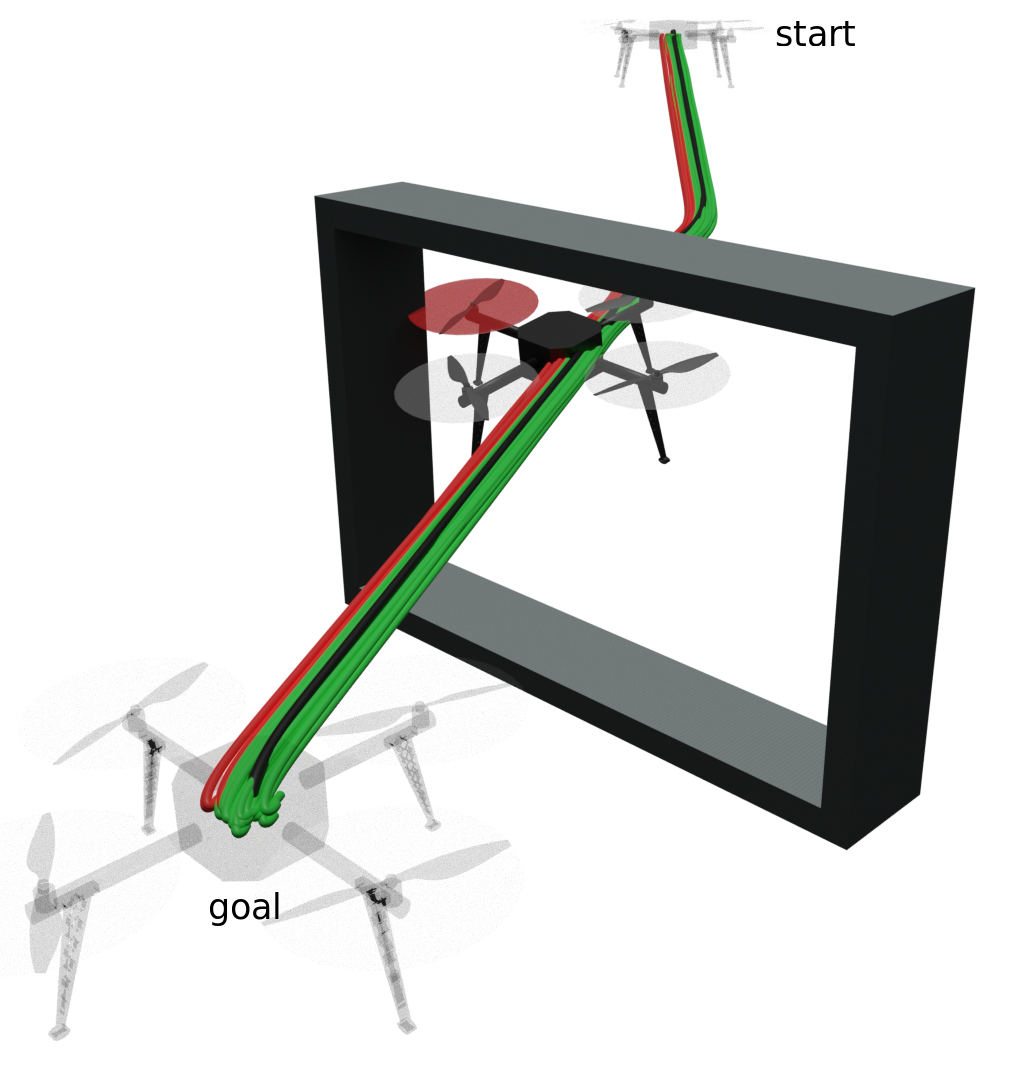
\includegraphics[width=0.4\linewidth]{figures/robust_accurate/simu_RRTstar_notube.png} }}%
    \subfloat[\centering R-SARRT$^*$]{{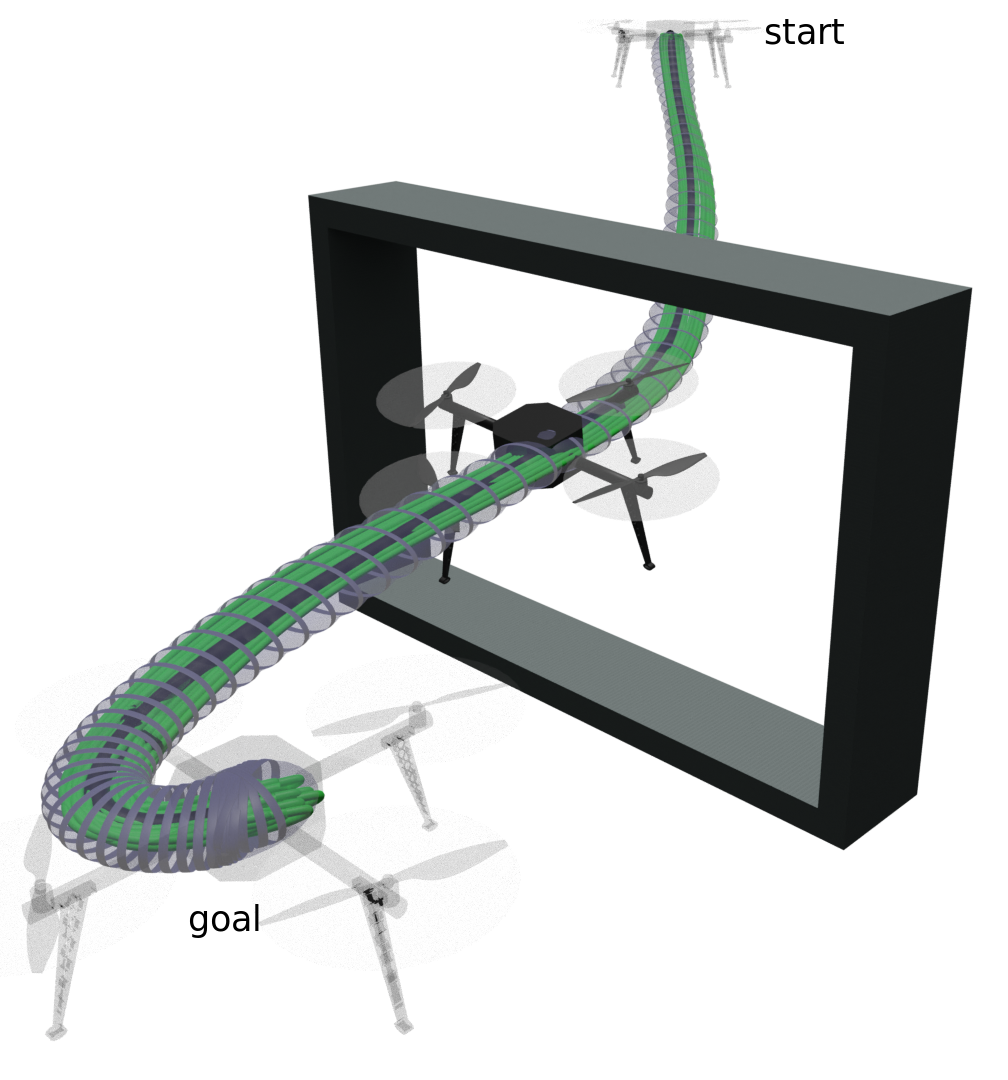
\includegraphics[width=0.4\linewidth]{figures/robust_accurate/simu_SARRTstar.png} }}%
    \caption{Planned trajectory (black) produced by a (a) RRT$^*$ and our (b) R-SARRT$^*$. 
    Simulated trajectories under uncertainty are displayed in green in the case of success, and in red in the case of a crash.}%
    \label{fig: simu window}%
\end{figure}

\begin{figure} [h]
    \centering
    
    \subfloat[\centering ]{{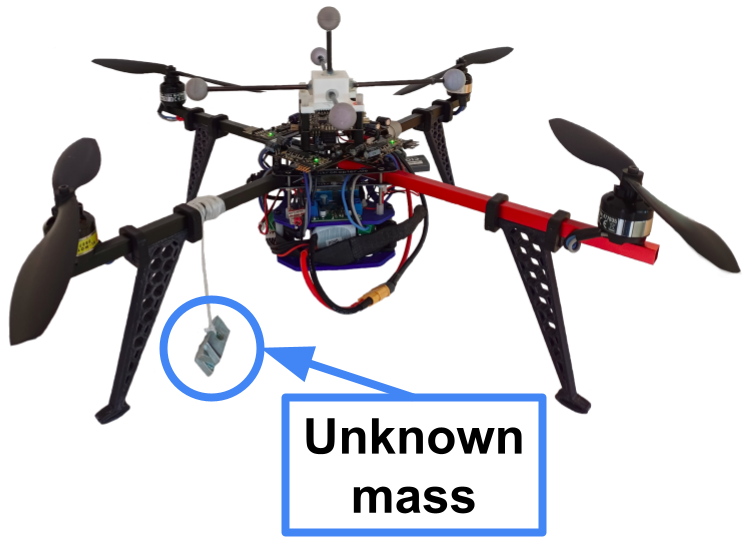
\includegraphics[width=0.42\linewidth]{figures/robust_accurate/drone_window.png} }\label{fig: drone_mass}}%
    \subfloat[\centering ]{{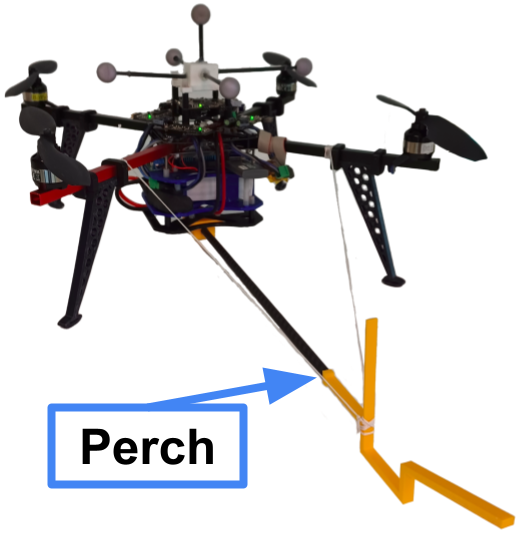
\includegraphics[width=0.3\linewidth]{figures/robust_accurate/drone_perch.png}} \label{fig: drone_perch}}%
    
    \caption{Quadrotor setups for the two scenarios considered for the experimental validation. (a) a drone equipped with a random mass to perform a robust navigation through a window (b) a drone equipped with a perch to catch the rings.}%
    \label{fig: exp setup}%
\end{figure}

\begin{figure} [h]
    \centering
    \subfloat[\centering RRT$^{*}$]{{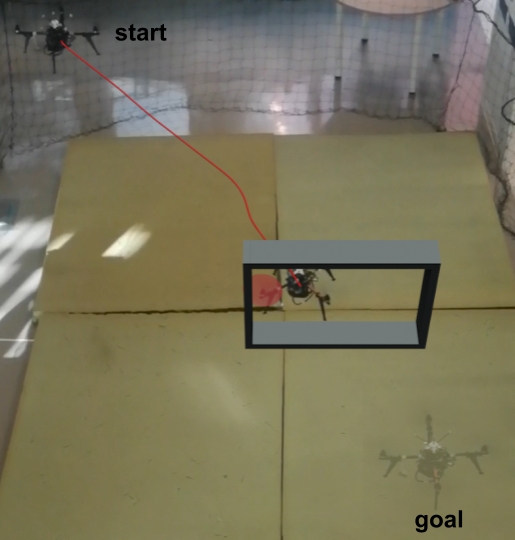
\includegraphics[width=0.4\linewidth]{figures/robust_accurate/exp_RRTstar.png} }}%
    \subfloat[\centering R-SARRT$^*$]{{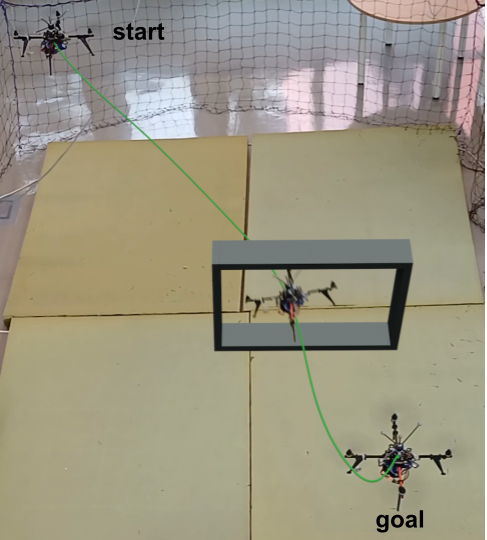
\includegraphics[width=0.378\linewidth]{figures/robust_accurate/exp_SARRTstar.png} }}%
    \caption{Experimental execution by a quadrotor with uncertainty of trajectories planned by  RRT$^*$ (a) and  R-SARRT$^*$ (b). Both trajectories are executed with the same uncertainty and a virtual collision is found in the RRT$^*$ case while the R-SARRT$^*$ execution is robust.}%
    \label{fig: exp window}%
\end{figure}

In this experiment, a non-robust trajectory planned by RRT$^*$ and a robust one planned by R-SARRT$^*$ were executed ten times, using the same masses and attachment points between the two algorithms.
All trajectories were planned offline on a remote computer. To make the robot execute them, the geometric controller~\cite{cLee} ran online on the quadrotor's onboard computer, tracking the trajectories provided as input. The robot state was measured using a motion capture system with millimeter accuracy, ensuring that the only source of uncertainty was the attached unknown mass.
Fig.\ref{fig: exp window} illustrates the experimental execution of a non-robust RRT$^*$ trajectory and a robust R-SARRT$^*$ trajectory. 
The figure shows the recorded executions within a virtual environment to detect virtual collisions, thus mitigating the risk of real crashes and damages to the robot.
The experimental results confirm the simulation observations, providing an overall success rate of 100\% in the case of the robust trajectory computed with R-SARRT$^*$, against 40\% for the classic RRT$^*$.

%%%%%%%%%%%%%%%%%%%%%%%%%%%%%%%%%%%%%%%%%%%%%%%%%%%%%%%%%%%%%%%%%%%%%%%%%%%%%%%%%%%%%%%%%%%%%%%%%%%%
\subsection{Accuracy optimization} \label{sec:AccOptSimu}

\begin{figure} [t]
    \centering
    {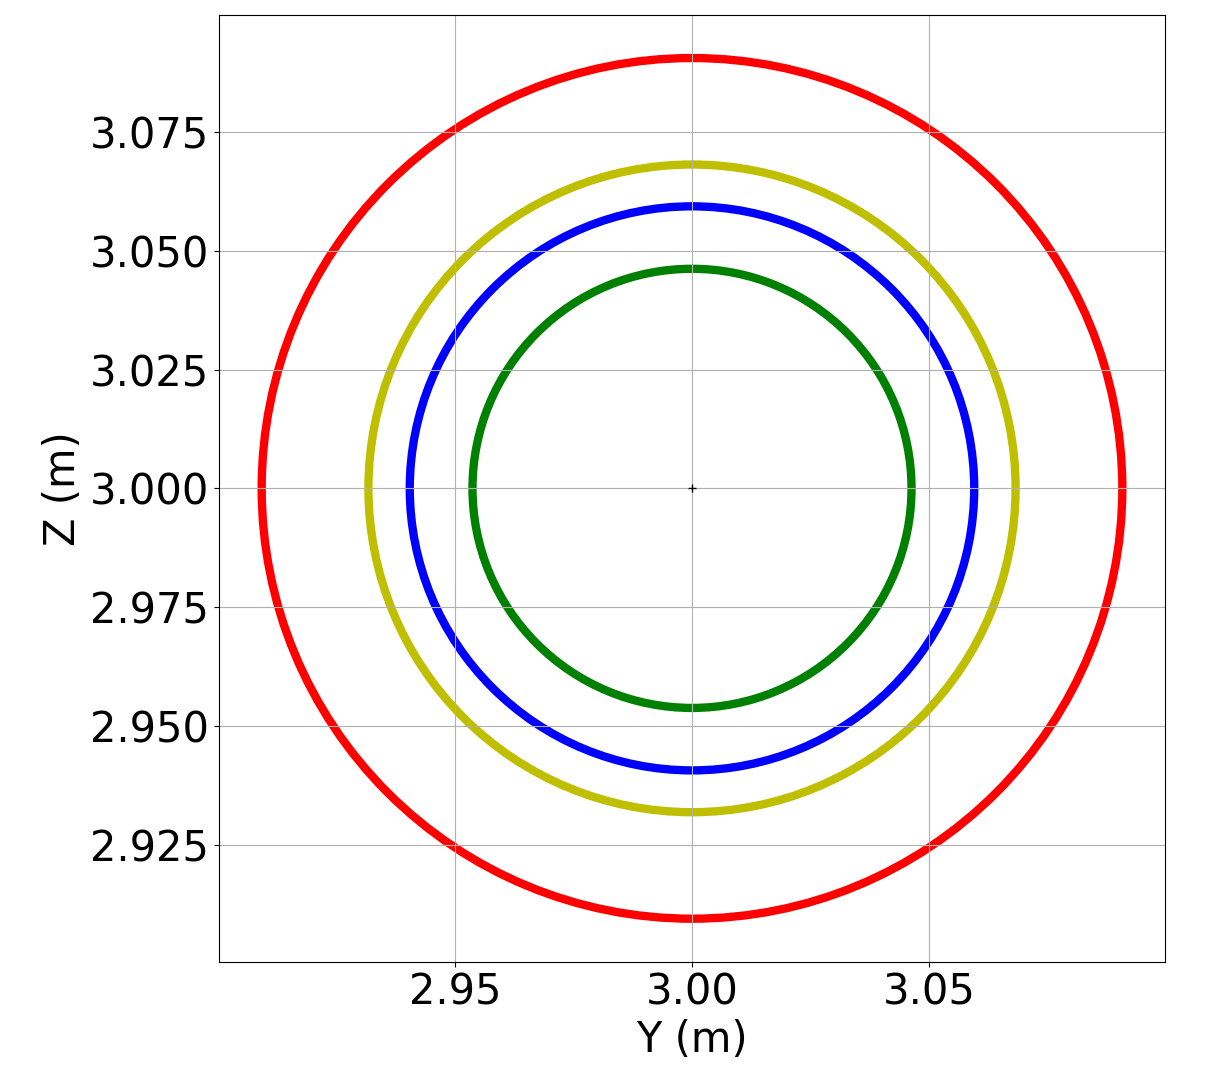
\includegraphics[width=0.5\linewidth]{figures/robust_accurate/accuracy_opti.png} }%
    \caption{Example of uncertainty ellipsoid without optimization (red), with local trajectory optimization (yellow), with gains optimization (blue), and with local trajectory and gains optimization at the same time (green).}%
    \label{fig: Acc opti}%
\end{figure}

We implemented the A-Optim method of Sect.\ref{sec:AOptim} by using a robust version of the random shortcut algorithm \cite{cShortcut} and \eqref{eq: cost} as cost function to be optimized, where the radii of interest are the ones along the $\boldsymbol{x}$, $\boldsymbol{\rho}$ and $\boldsymbol{\omega}$ components of $\boldsymbol{q}$.
At each iteration of this method, a shortcut is attempted between two states of the input trajectory that are randomly sampled together with the controller gain values, sampled between 50\% and 150\% of their nominal values.
Fig.\ref{fig: Acc opti} motivates why we optimized both the trajectory and the controller gains at the same time in the A-Optim function in order to minimize uncertainty for a given point, as mentioned in Sec.\ref{sec:RASAMP}. In fact, these results corroborate the findings of \cite{AliIROS}, but this time by employing a sampling-based motion planner that considers obstacles in the environment.

\section{Experimental validation} \label{sec:Experimental}
\subsection{Robust planning} \label{sec:RobustPlanExp}

\subsection{Accuracy optimization} \label{sec:AccOptExp}

\begin{figure} [t]
    \begin{subfigure}{0.63\linewidth}
      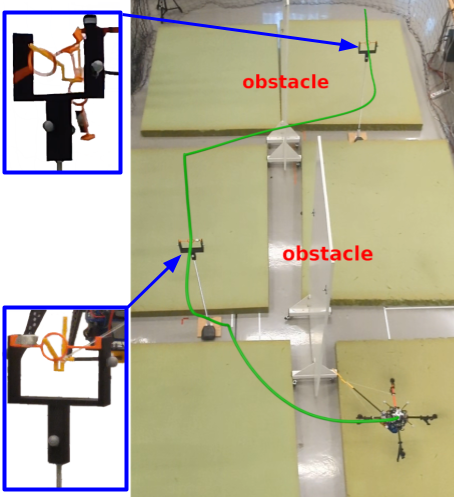
\includegraphics[width=\linewidth]{figures/robust_accurate/ring_opti_v1.png}
    \end{subfigure}\hfill
    \begin{subfigure}{0.37\linewidth}
        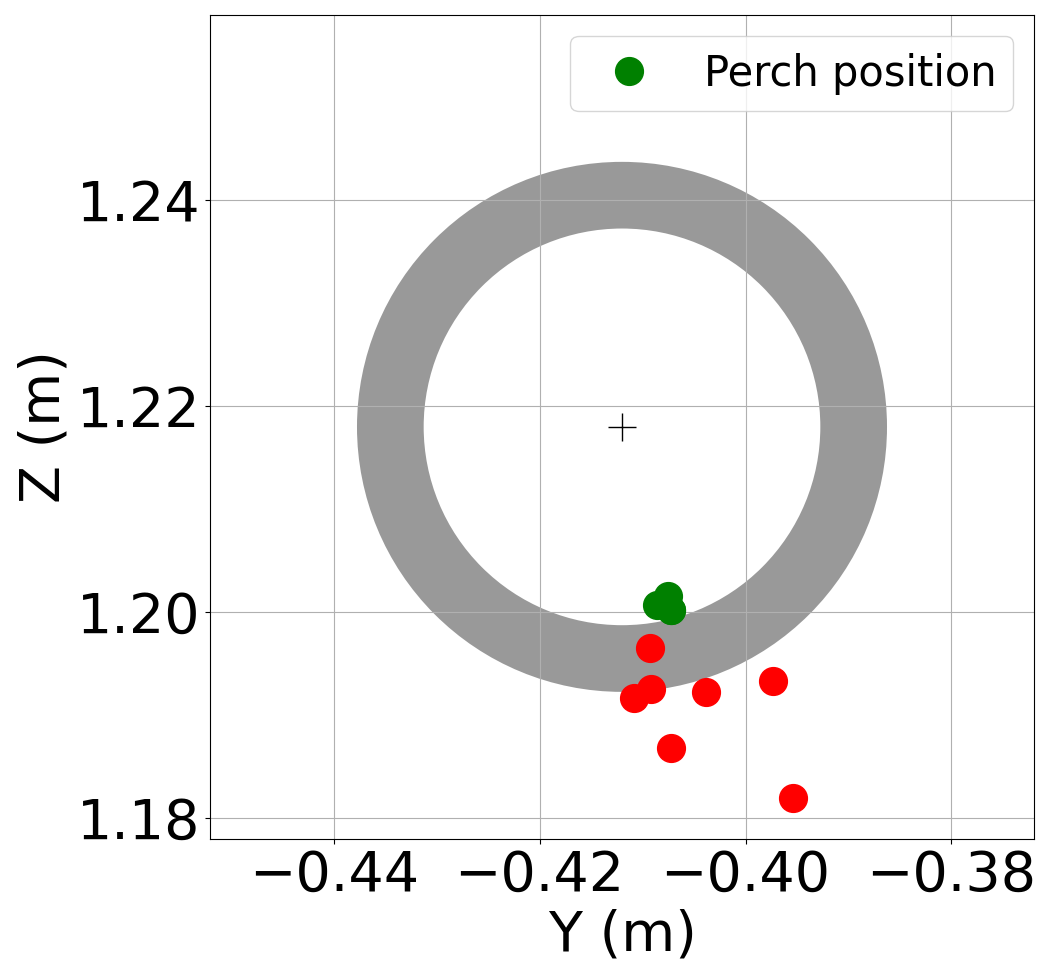
\includegraphics[width=\linewidth]{figures/robust_accurate/Exp_ring_no_opti_full_zoom.png}
        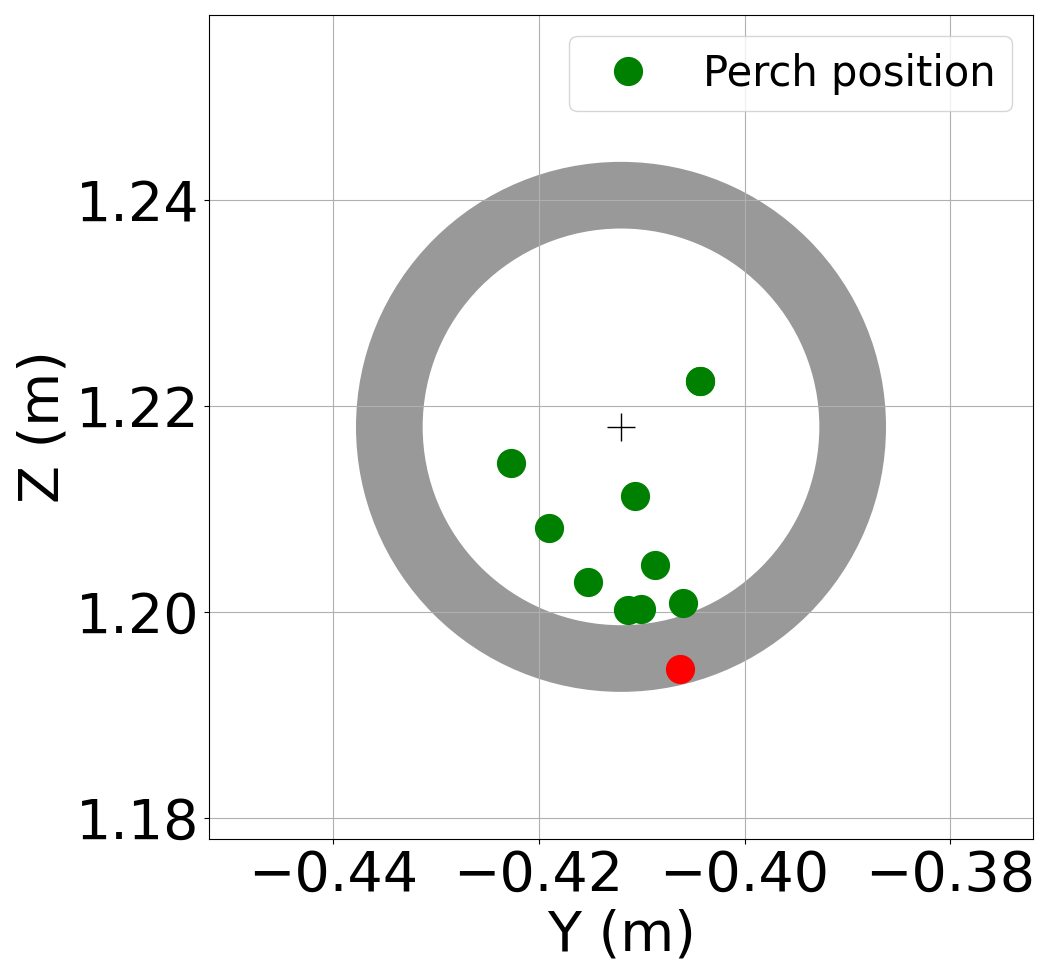
\includegraphics[width=\linewidth]{figures/robust_accurate/Exp_ring_opti_full_zoom.png}
      \end{subfigure}\hfill
      
    \caption{Experimental validation of the ``ring catching'' scenario with a perch-equipped drone (left) with the position of the perch end-effector at the second ring location over 10 trajectories non accuracy optimized (top right) and accuracy optimized (bottom right).}
    \label{fig: exp ring}
  \end{figure}

We evaluated our complete framework with the accuracy optimization in a scenario that involves the in-flight retrieval of two 2cm radius rings in a cluttered environment using a drone equipped with a perch (see Fig.\ref{fig: drone_perch}) in a (near) time optimal way.
The experimental setup is shown in Fig.\ref{fig: exp ring}.
When the first ring is caught it becomes part of the drone and modifies the overall mass/inertia and center of mass of the system in an unmodeled way. 
A success is characterized by the recovery of both rings, otherwise we consider the execution as a failure.

We executed 10 trajectories using a vanilla (non-robust) RRT$^*$ planner and the RA-SARRT$^*$ algorithm, both of which optimize the trajectory time.
The RRT$^*$ does not use the A-Optim method to optimize accuracy while the RA-SARRT$^*$ does, in addition to guaranteeing the robustness.
The offline optimization in A-Optim aimed at minimizing the uncertainty at the location of the two rings.
Fig.~\ref{fig: exp ring} shows the perch end-effector position at the second ring location in the non-optimized case and in the optimized one. 
In the latter case, the perch tip is closer to the reference point in the middle of the ring than in the former case. This translates into a higher success rate of nine out of ten attempts to catch the ring with the optimized approach, against only three times out of ten for the non-optimized case.
However, given the chosen system and controller parameters, there is no guarantee that the computed tube will be enclosed in within the ring.
This explains why we still encounter one failure in the optimized case.
Overall, the experimental results show a success rate of 90\% for RA-SARRT$^*$ against only 30\% for RRT$^*$.

%%%%%%%%%%%%%%%%%%%%%%%%%%%%%%%%%%%%%%%%%%%%%%%%%%%%%%%%%%%%%%%%%%%%%%%%%%%%%%%%%%%%%%%%%%%%%%%%%%%%
\section{Conclusion} \label{sec:Conclusion}

We have presented a motion planner able to generate trajectories that are both robust and accurate in the presence of model uncertainties for a variety of robot/controller pair. The proposed planner leverages a GRU-based learning approach that quickly and accurately estimates the control inputs and the sensitivity-based uncertainty tubes of the state and of the inputs. 
The results on a quadrotor robot confirm the efficiency of the proposed learning method and highlight the benefit of its integration within a motion planner, resulting in a significant reduction of the planning times. 
Moreover, we showed that our framework is able to locally optimize the planned trajectory in order to minimize the size of the uncertainty tubes of the state at some desired locations, allowing the system to accurately perform a precision task. An experimental demonstration involving a quadrotor UAV in a ring-catching task allowed to validate the approach in real conditions. Future works will focus on considering uncertainties not only in the dynamic model, by extending the computation of the tubes for state estimation uncertainties. 
Furthermore, we aim to expand the capabilities of the neural network to learn the optimal controller gains.
